%%%%%%%%%%%%%%%%%%%%%%%%%%%%%%%%%%%%%%%%%%%%%%%%%%%%%%%%%%%%%%%%%%%%%%%%%%%%%%%%%%
\begin{frame}[fragile]\frametitle{}
\begin{center}
{\Large TensorFlow Quantum}
\end{center}
\end{frame}

%%%%%%%%%%%%%%%%%%%%%%%%%%%%%%%%%%%%%%%%%%%%%%%%%%%%%%%%%%%
 \begin{frame}[fragile]\frametitle{Introduction}
 
\begin{itemize}
\item   TensorFlow Quantum library is an extension of TensorFlow 
\item  Quantum algorithms could speed up linear algebra operations, such as the calculation of eigenvalues needed for Machine Learning algorithms such as PCA.
\item But the quantum hardware is still not ready to run these algorithms. it is  still in the
NISQ (noisy intermediate scale quantum) era lacking sufficient noise tolerance to reach
scale for fault tolerance enabling error correction.
\item Imp to note that quantum neural networks are useful on quantum information such as simulated atomic systems or as may be registered with a quantum sensor etc.
\item  Otherwise classical networks are as a rule expected to train models either quicker or with better performance metrics.
\item Quantum
information differs from classical information due to the use of complex numbers as well
as the constraints imposed on matrix elements such as to ensure probability of
measurements sum to unity etc.
\item So QML is not for all, but for niche applications.
\end{itemize}

	
\tiny{(Ref: QML: Learning with TensorFlow Quantum - Nicholas Teague)}

\end{frame}

%%%%%%%%%%%%%%%%%%%%%%%%%%%%%%%%%%%%%%%%%%%%%%%%%%%%%%%%%%%
 \begin{frame}[fragile]\frametitle{Differences}
 
\begin{itemize}
\item  Neural Networks have layers, weights and activations one after another
\item Quantum Neural Networks need  input data embedded into quantum bits,
aka qubits, and so any operations applied onto that form will need to be conducted by
aggregations of quantum gates applied sequentially to and between those qubits
through the progression of time steps. 
\item With each of these gate operations, we’ll be
rotating the superposition state around an axis of those qubits’ ``Bloch spheres''.
\end{itemize}

\begin{center}
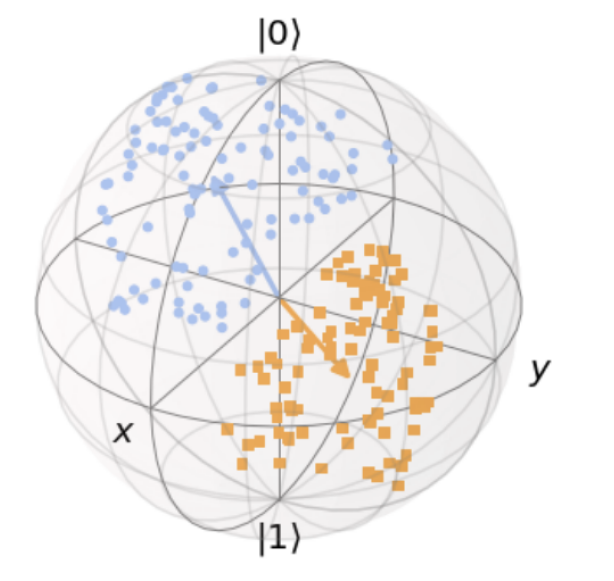
\includegraphics[width=0.3\linewidth,keepaspectratio]{bloch}
\end{center}
	
	
\tiny{(Ref: QML: Learning with TensorFlow Quantum - Nicholas Teague)}

\end{frame}

%%%%%%%%%%%%%%%%%%%%%%%%%%%%%%%%%%%%%%%%%%%%%%%%%%%%%%%%%%%
 \begin{frame}[fragile]\frametitle{Differences}
 
\begin{itemize}
\item  quantum algorithms are means to craft by such gate rotations a
shaped superposition of collective qubit states such that the probabilistic measurement
operations on the returned qubit states are more likely to collapse to classical states
corresponding to some desired output. 
\item The desired output state may correspond to the labels of a
supervised training operation.
\end{itemize}

\begin{center}
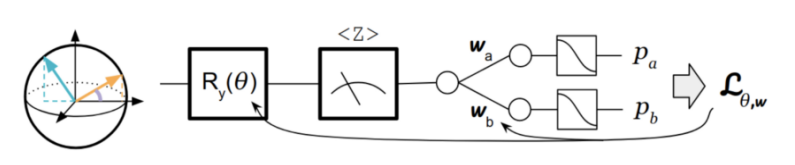
\includegraphics[width=0.8\linewidth,keepaspectratio]{qnn}
\end{center}
	
\begin{itemize}
\item  Question: if we’re not using layered neurons of weights and activation functions, how can this
be considered a neural network?
\item Answer: For our qubit states, the corollary to neural network weights will be parameterized gate applications, where these parameters control the magnitude or direction of Bloch sphere rotations.
\end{itemize}
	
\tiny{(Ref: QML: Learning with TensorFlow Quantum - Nicholas Teague)}

\end{frame}

%%%%%%%%%%%%%%%%%%%%%%%%%%%%%%%%%%%%%%%%%%%%%%%%%%%%%%%%%%%
 \begin{frame}[fragile]\frametitle{Differences}
 
\begin{itemize}
\item  Each layer of gates only interacts with adjacent qubits
instead of all to all. 
\item This reduced information flow is compensated by the depth of
information capacity of multi-qubit superpositions.
\end{itemize}

\begin{center}
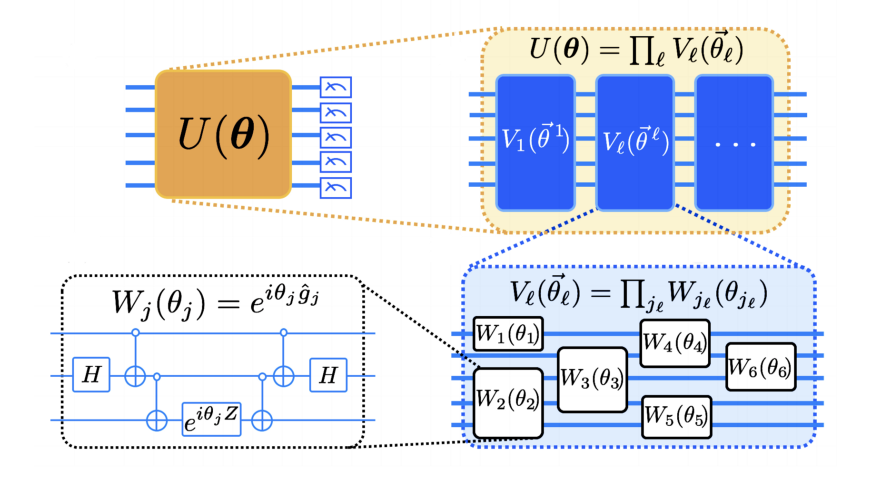
\includegraphics[width=0.6\linewidth,keepaspectratio]{qnn1}
\end{center}
	
\begin{itemize}
\item  The realized gated network can then be given a form of supervised training to fit the
parameterized gate sets to result in a returned superposition more aligned with our
target state as a function of inputs.
\end{itemize}
	
\tiny{(Ref: QML: Learning with TensorFlow Quantum - Nicholas Teague)}

\end{frame}

%%%%%%%%%%%%%%%%%%%%%%%%%%%%%%%%%%%%%%%%%%%%%%%%%%%%%%%%%%%
 \begin{frame}[fragile]\frametitle{Differences}
 
\begin{itemize}
\item  However we may find that these parameterized gates
on their own are insufficient to fully capture the breadth of transformation function
representations, especially considering the necessity of overcoming noisy hardware. 
\item The
architectures considered in the TensorFlow Quantum paper address this by integrating
classical networks commixed with the parameterized gates, in what they refer to as
hybrid quantum classical neural networks (HQCNN).
\end{itemize}

\begin{center}
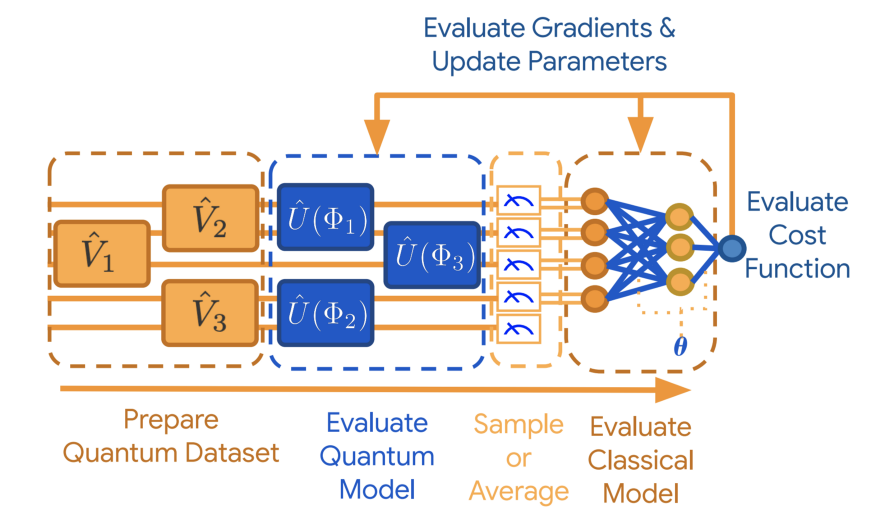
\includegraphics[width=0.6\linewidth,keepaspectratio]{qnn2}
\end{center}
	

\tiny{(Ref: QML: Learning with TensorFlow Quantum - Nicholas Teague)}

\end{frame}

%%%%%%%%%%%%%%%%%%%%%%%%%%%%%%%%%%%%%%%%%%%%%%%%%%%%%%%%%%%
 \begin{frame}[fragile]\frametitle{Differences}
 
\begin{itemize}
\item   The output statistics from measurement operations can be fed
into a classical network to translate those states to a consolidated prediction.
\item  the parameters of the gates could themselves be derived as a function of a classic neural network, in fact the interplay between quantum and classic network
channels could become quite elaborate, such as with alternating layer types between
quantum and classical or other structured flows.
\item  This kind of wholly different form of
parameterization could be integrated into a training loop. 
\end{itemize}

\begin{center}
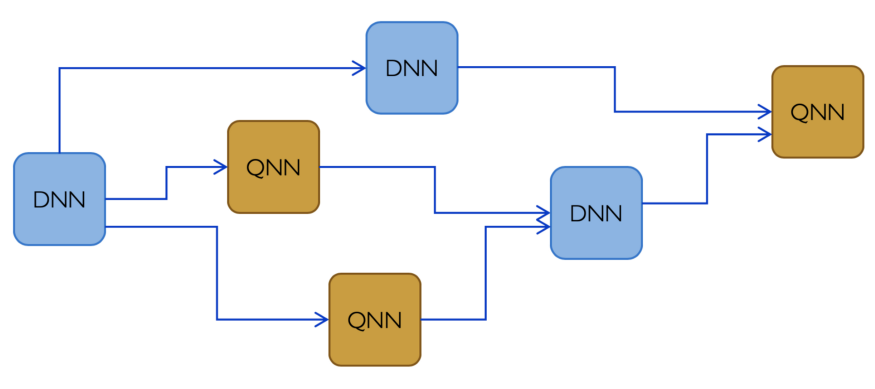
\includegraphics[width=0.6\linewidth,keepaspectratio]{qnn3}
\end{center}
	

\tiny{(Ref: QML: Learning with TensorFlow Quantum - Nicholas Teague)}

\end{frame}

%%%%%%%%%%%%%%%%%%%%%%%%%%%%%%%%%%%%%%%%%%%%%%%%%%%%%%%%%%%
 \begin{frame}[fragile]\frametitle{Differences}
 
\begin{itemize}
\item  The chain rule of backpropagation doesn’t directly translate to quantum primitives.
However, there is a very clean solution realized by the simple modularity inherent in the
networks.
\item In other words, if in a forward pass the returned measurements from a
quantum network are fed as input to a classical network, then in the backward pass we
can simply apply the returned gradients from the classical network as input to the
gradient calculations of the quantum network. Modular. 
\end{itemize}

\begin{center}
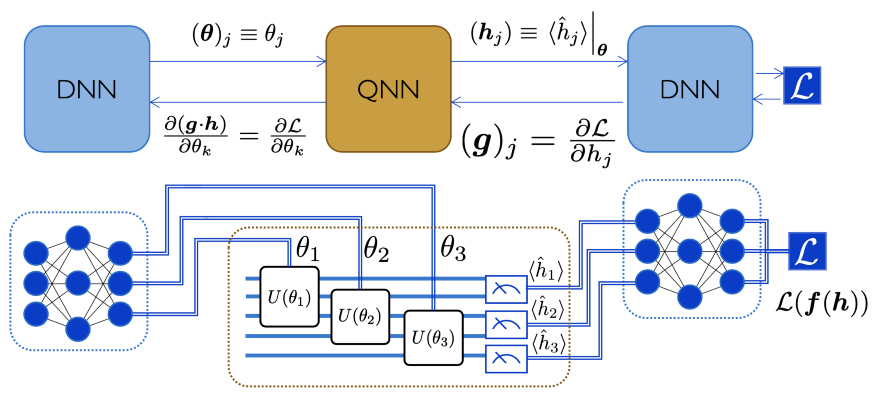
\includegraphics[width=0.6\linewidth,keepaspectratio]{qnn4}
\end{center}
	

\tiny{(Ref: QML: Learning with TensorFlow Quantum - Nicholas Teague)}

\end{frame}

%%%%%%%%%%%%%%%%%%%%%%%%%%%%%%%%%%%%%%%%%%%%%%%%%%%%%%%%%%%
 \begin{frame}[fragile]\frametitle{Introduction}
 
\begin{itemize}
\item  While a normal Turing machine can only perform one calculation at a time, a quantum Turing machine can perform many calculations at once.
\item  TFQ adds the ability to process quantum data, consisting of both quantum circuits and quantum operators. 
\end{itemize}

\begin{center}
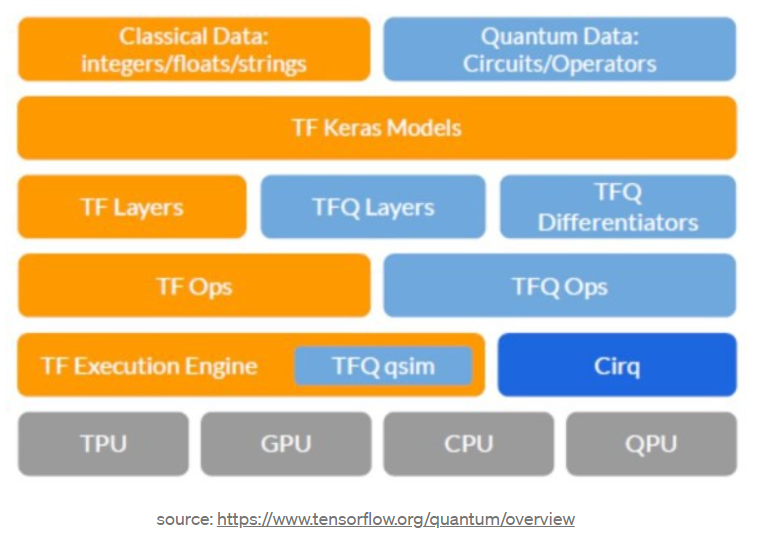
\includegraphics[width=0.6\linewidth,keepaspectratio]{tfq}
\end{center}
	
	
\tiny{(Ref: TensorFlow Quantum: beauty and the beast  - Shubham Goyal)}

\end{frame}

%%%%%%%%%%%%%%%%%%%%%%%%%%%%%%%%%%%%%%%%%%%%%%%%%%%%%%%%%%%
 \begin{frame}[fragile]\frametitle{TFQ Steps}
 
 TFQ steps to train and build QML models:
 
\begin{itemize}
\item  Prepare a quantum dataset: Quantum data is loaded as tensors, specified as a quantum circuit written in Cirq. The tensor is executed by TensorFlow on the quantum computer to generate a quantum dataset.
\item  Evaluate a quantum neural network model: prototype a quantum neural network using Cirq that will be embedded inside of a TensorFlow compute graph.
\item  Sample or Average: This step leverages methods for averaging over several runs involving steps (1) and (2).
\item  Evaluate a classical neural networks model: This step uses classical deep neural networks to distill such correlations between the measures extracted in the previous steps.
\item  Evaluate Cost Function: Similar to traditional machine learning models, TFQ uses this step to evaluate a cost function.
\item  Evaluate Gradients \& Update Parameters.
\end{itemize}

	
\tiny{(Ref: TensorFlow Quantum: beauty and the beast  - Shubham Goyal)}

\end{frame}

%%%%%%%%%%%%%%%%%%%%%%%%%%%%%%%%%%%%%%%%%%%%%%%%%%%%%%%%%%%
 \begin{frame}[fragile]\frametitle{QML Learning}
 

\begin{itemize}
\item  In quantum neural networks we’ll be feeding our input data embedded into quantum bits, aka qubits, and so any operations applied onto that form will need to be conducted by aggregations of quantum gates applied sequentially to and between those qubits through the progression of time steps. With each of these gate operations, we’ll be rotating the superposition state around an axis of those qubits’ “Bloch spheres”.
\item Quantum algorithms are means to craft by such gate rotations a shaped superposition of collective qubit states such that the probabilistic measurement operations on the returned qubit states are more likely to collapse to classical states corresponding to some desired output.
\item  Each layer of gates only interacts with adjacent qubits instead of all to all. This reduced information flow is compensated by the depth of information capacity of multi-qubit superpositions.

\end{itemize}

	
\tiny{(Ref: QML Learning with TensorFlow Quantum - Nicholas Teague)}

\end{frame}

%%%%%%%%%%%%%%%%%%%%%%%%%%%%%%%%%%%%%%%%%%%%%%%%%%%%%%%%%%%
 \begin{frame}[fragile]\frametitle{QML Learning}
 

\begin{itemize}
\item The realized gated network can then be given a form of supervised training to fit the parameterized gate sets to result in a returned superposition more aligned with our target state as a function of inputs. 
\item  The chain rule of backpropagation doesn’t directly translate to quantum primitives. However, there is a very clean solution realized by the simple modularity inherent in the networks. In other words, if in a forward pass the returned measurements from a quantum network are fed as input to a classical network, then in the backward pass we can simply apply the returned gradients from the classical network as input to the gradient calculations of the quantum network.
\end{itemize}

	
\tiny{(Ref: QML Learning with TensorFlow Quantum - Nicholas Teague)}

\end{frame}